\documentclass[compress,12pt]{beamer}

\usetheme{Arguelles}
\usepackage{graphicx}
\usepackage{caption}
%\usepackage[spanish,es-noshorthands]{babel}
\usepackage{babel} 
\usepackage[pages=some]{background}
\usepackage{tikz}
\usepackage{tikz-cd}
\usepackage{amsmath,amssymb,latexsym,amscd} 
\usepackage[all,cmtip]{xy}
\usepackage{fancyhdr}
\usepackage{mathalfa}
\usepackage{mathrsfs}
\usetikzlibrary{babel}
\usepackage{hyperref}
\usepackage{ragged2e}
\usepackage{wasysym}
\usepackage{tikz}
\usetikzlibrary{arrows.meta,calc,positioning,overlay-beamer-styles,shadows.blur}
%\hypersetup{colorlinks=true,linkcolor=blue,citecolor=brown,linktocpage=true,pagebackref=true,hyperindex=true}
\pagenumbering{arabic}

\DeclareMathOperator{\op}{op}
\DeclareMathOperator{\pt}{pt}
\DeclareMathOperator{\spec}{spec}
\DeclareMathOperator{\Fit}{Fit}
\DeclareMathOperator{\Pth}{P}
\DeclareMathOperator{\Frm}{Frm}
\DeclareMathOperator{\Top}{Top}
\DeclareMathOperator{\Ord}{Ord}
\DeclareMathOperator{\Obj}{Obj}
\DeclareMathOperator{\Hom}{Hom}

\title{The patch frame}
\subtitle{and some separation axioms in Frm}
\event{58° Congreso Nacional de la SMM}
\date{Interacciones entre Topología, Álgebra y Categorías}
\author{Juan Carlos Monter Cortés}
\institute{Universidad de Guadalajara}
\email{juan.monter2902@alumnos.udg.mx}

%\homepage{www.mywebsite.com}
%\github{username}

\begin{document}

\frame[plain]{\titlepage}

%\begin{frame}{Contenido}
%\tableofcontents %Imprime la tabla de contenido
%\end{frame}
\section{Background and motivation}
\begin{frame}{A little example}
Let $S=\mathbb{R}$ be with the topologies
\[
\mathcal{O}_lS=\{(-\infty, a)\},\quad  \mathcal{O}_mS=\{(a,b)\}, \quad \mathcal{O}_nS=\{[a,b)\},
\]
where $a,b\in S$. Then
\[
\mathcal{O}_lS \hookrightarrow \mathcal{O}_mS \hookrightarrow \mathcal{O}_nS
\]

We can see that 
\[
\mathcal{O}_l^pS=\mathcal{O}_mS\simeq P\mathcal{O}_lS\quad\mbox{ y }\quad\mathcal{O}_l^fS=\mathcal{O}_nS\simeq N\mathcal{O}_lS,
\]
that is, 
\[
\mathcal{O}_lS=A\rightarrow PA\hookrightarrow NA
\]
\end{frame}

\begin{frame}{The patch construction}
\centering
\resizebox{\textwidth}{!}{%
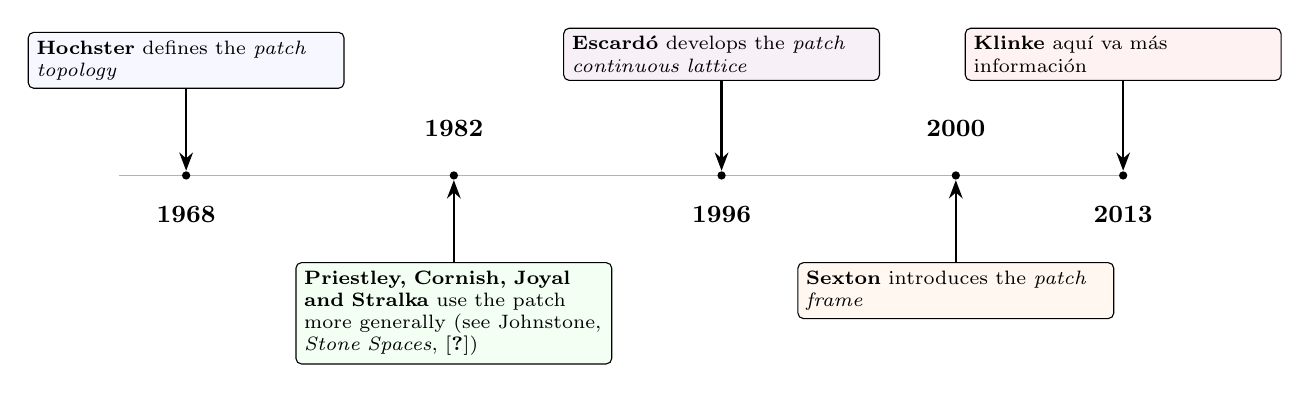
\begin{tikzpicture}[
  x=0.85cm, y=1cm,
  >=Stealth,
  year/.style={font=\small\bfseries},
  base/.style={
    draw, rounded corners=2pt, fill=white, align=left, inner sep=3pt,
    font=\scriptsize, text width=3.8cm
  },
  E1968/.style={base, fill=blue!3},
  E1982/.style={base, fill=green!5},
  E1996/.style={base, fill=violet!6},
  E2000/.style={base, fill=orange!6},
  E2013/.style={base, fill=red!5},
  tick/.style={circle, fill, minimum size=3pt, inner sep=0pt},
  axis/.style={line width=0.6pt, gray!60}
]

% --- Eje base
\draw[axis] (0,0) -- (15,0);

% --- Coordenadas
\coordinate (p68) at (1,0);
\coordinate (p82) at (5,0);
\coordinate (p96) at (9,0);
\coordinate (p00) at (12.5,0);
\coordinate (p13) at (15,0);

% --- Años (1968, 1996 abajo; 1982, 2000, 2013 arriba)
\node[tick, visible on=<1->] at (p68) {};
\node[year, visible on=<1->] at ($(p68)+(0,-0.5)$) {1968};

\node[tick, visible on=<2->] at (p82) {};
\node[year, visible on=<2->] at ($(p82)+(0,0.6)$) {1982};

\node[tick, visible on=<3->] at (p96) {};
\node[year, visible on=<3->] at ($(p96)+(0,-0.5)$) {1996};

\node[tick, visible on=<4->] at (p00) {};
\node[year, visible on=<4->] at ($(p00)+(0,0.6)$) {2000};

\node[tick, visible on=<5->] at (p13) {};
\node[year, visible on=<5->] at ($(p13)+(0,-0.5)$) {2013};

% --- Eventos alternados
\node[E1968, anchor=south, visible on=<1->] (e1968) at ($(p68)+(0,1.1)$)
  {\textbf{Hochster} defines the \emph{patch topology}};

\node[E1982, anchor=north, visible on=<2->] (e1982) at ($(p82)+(0,-1.1)$)
  {\textbf{Priestley, Cornish, Joyal and Stralka} use the patch more generally (see Johnstone, \emph{Stone Spaces}, \cite{P.T.})};

\node[E1996, anchor=south, visible on=<3->] (e1996) at ($(p96)+(0,1.2)$)
  {\textbf{Escard\'o} develops the \emph{patch continuous lattice}};

\node[E2000, anchor=north, visible on=<4->] (e2000) at ($(p00)+(0,-1.1)$)
  {\textbf{Sexton} introduces the \emph{patch frame}};

\node[E2013, anchor=south, visible on=<5->] (e2013) at ($(p13)+(0,1.2)$)
  {\textbf{Klinke} aquí va más información};

% --- Flechas verticales
\draw[->, thick, visible on=<1->] (e1968.south) -- ($(p68)+(0,0.06)$);
\draw[->, thick, visible on=<2->] (e1982.north) -- ($(p82)+(0,-0.06)$);
\draw[->, thick, visible on=<3->] (e1996.south) -- ($(p96)+(0,0.06)$);
\draw[->, thick, visible on=<4->] (e2000.north) -- ($(p00)+(0,-0.06)$);
\draw[->, thick, visible on=<5->] (e2013.south) -- ($(p13)+(0,0.06)$);

\end{tikzpicture}%
}% end resizebox
\end{frame}

\begin{frame}[fragile]{Frame theory}
\[
\Frm= \left\{ \begin{array}{lc} \Obj: & (A, \leq, \wedge, \bigvee, 1, 0) \\ \\ \mbox{Arrows:} & f\colon A\to B  \end{array} \right.
\]

For $S\in \Top$,
\[
(\mathcal{O}S, \subseteq, \cap, \bigcup, S, \emptyset)\in \Frm
\]
Furthermore,
\[
\begin{tikzcd}
\Top \arrow[rr, "\mathcal{O}(\_)", bend left] &  & \Frm \arrow[ll, "\pt(\_)", bend left]
\end{tikzcd}
\]
is an adjunction.
\end{frame}

\begin{frame}{Packed spaces}
    $^pS=(S, \mathcal{O}^pS)$, where $\mathcal{O}^pS$ is gerated by
    \[
    \mbox{pbase}=\{U\cap Q'\mid U\in \mathcal{O}S, Q\in \mathcal{Q}S\}
    \]
\begin{block}{Definition}
$S\in \Top$ is \textbf{packed} if every compact (saturated) set is closed
\end{block}
\[
S \mbox{ is packed}\quad\iff\quad ^pS=S
\]

\[
T_2\Rightarrow \mbox{packed}\Rightarrow T_1
\]
\end{frame}

\begin{frame}{Patch trivial}
By \emph{Hoffman-Mislove theorem}\footnote{\textbf{Thm:} There is a bijective correspondence between $F\in A^\wedge$ and $Q\in \mathcal{Q}S$}
\[
\mbox{Pbase}=\{u_a\wedge v_F\mid a\in A, F\in A^\wedge\}
\]
\begin{block}{Definition}
\begin{enumerate}
    \item The \textbf{patch frame} of $A\in \Frm$ $(PA)$, is the frame generated by Pbase
    \item $A$ is \textbf{patch trivial} if $A\simeq PA$.
\end{enumerate}
\end{block}

\footnotetext[0]{$F\in A^\wedge$ if $F$ is a filter in $A$ and $\forall\, X\subseteq A$, with $X$ directed, if $\bigvee X\in F$, then $a\in F$ for some $a\in X$.}
\footnotetext[0]{For $a\in A$, $u_a(x)=a\vee x$ and $v_a(x)=(a\succ x)$ are nuclei in $A$.}
\footnotetext[0]{$v_F=f^\infty$, where $f=\dot{\bigvee}\{v_a\mid a\in F\}$ }
\end{frame}

\begin{frame}{Tidy frames}
\begin{block}{Definition [\cite{R.S.3}, Def. 8.2.1]}
Let $A\in \Frm$, $F\in A^\wedge$ and $\alpha\in \Ord$ be. We say that:
\begin{enumerate}
    \item $F$ is $\alpha$-tidy if for $x\in F$, $d\vee x=1$, where
    \[
    d=d(\alpha)=f^\alpha(0).
    \]
    \item $A$ is $\alpha$-tidy if every $F\in A^\wedge$ is $\alpha$-tidy.
    \item $A$ is \textbf{tidy} if it is $\alpha$-tidy for some $\alpha\in \Ord$.
\end{enumerate}
\end{block}

\begin{block}{Proposition [\cite{R.S.3}, Lemma 8.2.2]}
\[
    A \mbox{ is tidy}\quad \iff\quad A \mbox{ is patch trivial}.
\]
\end{block}
\end{frame}

\begin{frame}[plain,standout]
      \centering{
      \Huge{Objectives}}
      \begin{enumerate}
        \item Understand tidy frames in more detail.
        \item To explore the relationship with some separation axioms in $\Frm$.
        \item Provide tools to study the tidy frames.
        \item Give examples.
      \end{enumerate}
\end{frame}

\begin{frame}[fragile]{Separation axioms in Frm}
\[\begin{tikzcd}
	&& {\mathbf{(reg)}} \\
	{\mathbf{(fit)}} && {\mathbf{(sH)}} && {\mathbf{(H)}+\mathbf{(sfit)}} \\
	{\mathbf{(sfit)}} && {T_1} && {\mathbf{(H)}}
	\arrow[Rightarrow, from=1-3, to=2-1]
	\arrow[Rightarrow, from=1-3, to=2-3]
	\arrow[Rightarrow, from=1-3, to=2-5]
	\arrow[Rightarrow, from=2-1, to=3-1]
	\arrow[Rightarrow, from=2-1, to=3-3]
	\arrow[dotted, no head, from=2-3, to=2-1]
	\arrow[dotted, no head, from=2-3, to=2-5]
	\arrow[dotted, no head, from=2-3, to=3-1]
	\arrow[Rightarrow, from=2-3, to=3-3]
	\arrow[Rightarrow, from=2-3, to=3-5]
	\arrow[Rightarrow, from=2-5, to=3-5]
	\arrow[dotted, no head, from=3-1, to=3-3]
	\arrow[Rightarrow, from=3-5, to=3-3]
\end{tikzcd}\]
\footnotetext[0]{$\forall\, a\nleq b\in A$, then }
\footnotetext[0]{\textbf{(reg):} $\exists \, x,y\in A$ such that $a\vee x=1, y\nleq b$ and $x\wedge y=0$.}
\footnotetext[0]{\textbf{(H):} $\exists\, c\in A$ such that $c\nleq a$ and $\neg c\leq b$.}
\footnotetext[0]{\textbf{(fit):} $\exists\, x,y\in A$ such that $x\vee a=1, y\nleq b$ and $x\wedge y\leq b$.}
\footnotetext[0]{\textbf{(sfit):} $\exists\, c\in A$ such that $c\vee a=1\neq c\vee b$.}
\footnotetext[0]{\textbf{(sH)} and $T_1$ are notion some different. All this can be found in \cite{J.P.2}.}
\end{frame}

\begin{frame}{Properties of the tidy frames}
This is a summary of the properties that Sexton includes in \cite{R.S.3}
\begin{itemize}
\item In the spatial case ($A=\mathcal{O}S$),
\[
\begin{split}
\mathcal{O}S \mbox{ is 0-tidy } & \iff S=\emptyset \\
\mathcal{O}S \mbox{ is 1-tidy } & \iff S \mbox{ is }T_2 \\
\mathcal{O}S \mbox{ is tidy } & \iff S \mbox{ is packed and stacked}.
\end{split}
\]

\item For $A\in \Frm$ arbitrary
\[
\begin{split}
A\mbox{ is }\mathbf{(reg)} & \Rightarrow A \mbox{ is tidy}\\
A\mbox{ is }\mathbf{(fit)} & \Rightarrow A \mbox{ is tidy}\\
A\mbox{ is tidy } & \Rightarrow A\mbox{ is } T_1
\end{split}
\]
\end{itemize}
\end{frame}

\section{Some results}

\begin{frame}[fragile]{Some results}
If $(f\colon A\to B)\in \Frm$, $G\in A^\wedge$ and $F\in B^\wedge$, then
\[
b\in f[G]\iff f_*(b)\in G\quad\mbox{ and }\quad a\in f_*[F]\iff f(a)\in F.
\]
Also, if $F\in B^\wedge$, then $f_*(F)\in A^\wedge$.
\begin{block}{Proposition}
For $f^\infty$ and $f_j^\infty$ the nuclei associated to $F$ and $j_*F$, respectively, we have
\[
j\circ f_j^\infty\leq f^\infty \circ j
\]
\end{block}
\begin{proof}
By induction transfinite.
\end{proof}
\end{frame}

\begin{frame}{More properties of the tidy frames}
\begin{block}{Proposition}
If $A\in \Frm$ is tidy and $j\in NA$, then $A_j$ is tidy.
\end{block}
\begin{proof}
\begin{itemize}
\item We take $x\in F\in A_j^\wedge$ and $F\subseteq j_*[F]\in A^\wedge$.
\item For $f^\infty$ and $f_j^\infty$ as before, we have
\[
d=d(\alpha)\geq d_j(\alpha)=d_j
\]
\item Since $A$ is tidy, then $d_j\vee x=1$, for all $x\in j_*[F]$. In particular, for all $x\in F$.
\item Therefore, $d\vee x=1$.
\end{itemize}
\end{proof}

%\begin{block}{Proposition}
%If $A, B\in \Frm$ are tidy, then $A\oplus B$ is tidy.
%\end{block}
\end{frame}

\begin{frame}[fragile]
\begin{block}{Corollary}
If $A$ is $\mathbf{(sH)}$, $A$ is tidy.
\end{block}
\begin{proof}
In $\mathbf{(sH)}$ all compact quotient is closed.
\end{proof}

\[\begin{tikzcd}
	& {\mathbf{(H)}} \\
	{\mathbf{(reg)}} & {\mathbf{(sH)}} & {\text{Tidy}} \\
	& {\mathbf{(fit)}}
	\arrow[Rightarrow, dotted, from=1-2, to=2-3]
	\arrow[Rightarrow, from=2-1, to=1-2]
	\arrow[Rightarrow, from=2-1, to=2-2]
	\arrow[Rightarrow, from=2-1, to=3-2]
	\arrow[Rightarrow, from=2-2, to=1-2]
	\arrow[Rightarrow, from=2-2, to=2-3]
	\arrow[Rightarrow, from=3-2, to=2-3]
\end{tikzcd}\]
\end{frame}

\begin{frame}{Compact quotients}
  \[
  \mbox{Tidy} \iff \mbox{ P. trivial }\iff u_d=v_F
  \]

  \begin{block}{Theorem}
  Let $A\in \Frm$ and $j\in NA$. Then
  \[
    A_j \mbox{ is compact}\quad\iff\quad \nabla(j)\in A^\wedge.
  \]
  \end{block}
  Then
  \[
  A_{u_d} \mbox{ is a closed quotient}\quad \mbox{ and }\quad A_{v_F} \mbox{ is a compact quotient.}
  \]
  If $A$ is tidy, we have a compact closed quotient.

\footnotetext[0]{$\nabla(j)=\{a\in A\mid j(a)=1\}$ is a filter in $A$ \emph{(Admissibility filter)}.}
\footnotetext[0]{With $\nabla(j)$ we can define a ``$\sim$'' in $NA$: $j\sim k\iff \nabla(j)=\nabla(k)$.}
\end{frame}

\begin{frame}{KC frames}
In \cite{A.W.}, Wilansky defines a space $S$ to be \textbf{KC} if every compact set is closed. 

\begin{block}{Definition}
$A\in \Frm$ is a \textbf{KC frame} if every compact quotient is closed.
\end{block}
\[
\mathbf{KC}\Rightarrow \mbox{Tidy}
\]
\begin{block}{Proposition}
If $A\in \Frm$ es $\mathbf{KC}$ and $j\in NA$, then $A_j$ is $\mathbf{KC}$.
\end{block}
\end{frame}

\begin{frame}
\begin{proof}
\begin{itemize}
  \item Consider $k\in NA_j$ such that $\nabla(k)\in A_j^\wedge$.
  \item If $\nabla(k)\in A_j^\wedge \Rightarrow j_*[\nabla(k)]\in A^\wedge$.
  \item We take $l=j_*\circ k\circ j\in NA$ and $\nabla(l)\in A^\wedge\Rightarrow l=u_a$ for some $a\in A$.
  \item Furthermore $a=k(j(a))$.
  \item For $x, b\in A_j$ with $b=j(a)$ we have $u_b(x)=k(x)$. 
\end{itemize}
\end{proof}

\footnotetext[0]{\textbf{Proposition:} For $j\in NA$ and $k\in NA_j$. If $\nabla(k)\in A_j^\wedge$, $\nabla(j_*kj)\in A^\wedge$.}
\end{frame}

\begin{frame}[fragile]
We can build the diagram (see \cite{H.S.V})
\[\begin{tikzcd}
	A && {A_F} \\
	&&& \mathcal{O}Q \\
	{\mathcal{O}S} && {\mathcal{O}S_\nabla}
	\arrow["{v_F}", from=1-1, to=1-3]
	\arrow["{U_A}"', from=1-1, to=3-1]
	\arrow["{\simeq }", from=1-3, to=2-4]
	\arrow["g", from=1-3, to=3-3]
	\arrow["{v_\nabla}"', from=3-1, to=3-3]
	\arrow["{\simeq }"', from=3-3, to=2-4]
\end{tikzcd}\]
What happens if A has property $\mathbf{(H)}$?

\footnotetext{$g=(u_A)_*\circ (v_\nabla)_{\mid A_F}$.}
\end{frame}

\begin{frame}
\begin{block}{Theorem}
Let $A$ be a frame with property $\mathbf{(H)}$ then for every $F\in A^\wedge$ with corresponding $Q\in \mathcal{Q}S$ compact we have
\[
\mathcal{O}Q\simeq \uparrow{Q'},
\]
that is, the frame of opens of the point space of $A_F$ is isomorphic to a compact
closed quotient of a Hausdorff space.
\end{block}
\end{frame}

\begin{frame}{Some examples}
\begin{itemize}
\item With the cofinite topology we look that $PA= NA$.
\item With the cocountable topology we look that $\pt NA\subseteq \pt PA$.
\item With a subregular topology on the real we have a 1-tidy frame that is not regular. 
\item With the maximal compact topology we have a 2-tidy frame that is not 1-tidy.
\item With the boss topology on a tree we look that exist $\alpha$-tidy frames.
\end{itemize}
\end{frame}


\End
\section*{\textsc{Referencias}}
\begin{frame}[allowframebreaks]
\frametitle{Bibliografía}
\begin{thebibliography}{20}\markboth{Bibliografía}{Bibliografía}

\bibitem{P.T.} P. T. Johnstone, \textit{Stone spaces}, Cambridge Studies in Advanced Mathematics, vol. 3, Cambridge University Press, Cambridge, 1982. MR 698074

\bibitem{J.M.} J. Monter; A. Zaldívar, \textit{El enfoque locálico de las reflexiones booleanas: un análisis en la categoría de marcos} [tesis de maestría], 2022. Universidad de Guadalajara.

\bibitem{P.S.} J. Paseka and B. Smarda, \textit{$ T_2 $-frames and almost compact frames.} Czechoslovak Mathematical Journal (1992), 42(3), 385-402.

\bibitem{J.P.} J. Picado and A. Pultr, \textit{Frames and locales: Topology without points}, Frontiers in Mathematics, Springer Basel, 2012.

\bibitem{J.P.2} J. Picado and A. Pultr, \textit{Separation in point-free topology}, Springer, 2021.

\bibitem{R.S.} RA Sexton, \textit{A point free and point-sensitive analysis of the patch assembly}, The University of Manchester (United Kingdom), 2003.

\bibitem{R.S.2} RA Sexton, \textit{Frame theoretic assembly as a unifying construct}, The University of Manchester (United Kingdom), 2000.

\bibitem{R.S.3} RA Sexton and H. Simmons, \textit{Point-sensitive and point-free patch constructions}, Journal of Pure and Applied Algebra \textbf{207} (2006), no. 2, 433-468.

\bibitem{H.S.} H. Simmons, \textit{An Introduction to Frame Theory}, lecture notes, University of Manchester. Disponible en línea en \url{https://web.archive.org/web/20190714073511/http://staff.cs.manchester.ac.uk/~hsimmons}.

\bibitem{H.S.R} H. Simmons, \textit{Regularity, fitness, and the block structure of frames.} Applied Categorical Structures 14 (2006): 1-34.

\bibitem{H.S.4} H. Simmons, \textit{The lattice theoretic part of topological separation properties}, Proceedings of the Edinburgh Mathematical Society, vol.~21, pp.~41--48, 1978.

\bibitem{H.S.V} H. Simmons, \textit{The Vietoris modifications of a frame}. Unpublished manuscript (2004), 79pp., available online at http://www. cs. man. ac. uk/hsimmons.

\bibitem{A.W.} A. Wilansky, \textit{Between T1 and T2}, MONTHLY (1967): 261-266.

\bibitem{A.Z.} A. Zaldívar, \textit{Introducción a la teoría de marcos} [notas curso], 2025. Universidad de Guadalajara.
\end{thebibliography}
\end{frame}

\end{document}